\documentclass[12pt]{article}
\usepackage{zed-csp}
\usepackage[top=2.5cm, bottom=2.5cm, left=3cm, right=3cm]{geometry}
\usepackage{graphicx}
\begin{document}

\begin{Huge}
\begin{center}
\begin{normalsize}
\textbf{MAKERERE 
\includegraphics[scale=0.5]{logo} UNIVERSITY }\\


\textbf{FACULTY OF COMPUTING AND INFORMATICS TECHNOLOGY} \\
\textbf{SCHOOL OF COMPUTING AND INFORMATICS TECHNOLOGY} \\
\textbf{DEPARTMENT OF COMPUTER SCIENCE} \\
\textbf{BACHELOR OF SCIENCE IN COMPUTER SCIENCE} \\
\textbf{YEAR 2} \\
\textbf{BIT 2207 RESEARCH METHODOLOGY} \\
\textbf{Course Work: Proposal Assignment }\\
\end{normalsize}
\end{center}
\end{Huge}

\begin{center}
\begin{tabular}{|l|l|l|c|}
\hline NAME  & REG NO & STD NO \\\hline

ABILA Raphael& 16/U/2673/PS & 216006923 \\\hline
MWAITA Joshua& 16/U/7890/PS & 216018350 \\\hline
NAKAFEERO Peninah&16/U/8463/PS & 216009254 \\\hline
OJIAMBO ABEX     & 16/U/10829/PS & 216013324 \\\hline
\end{tabular}
\paragraph{•}
Lecturer: ERNEST MWEBAZE \\
\paragraph{•}
9th March 2018

\end{center}

\newpage
\title{}\textbf{AUTOMATED WEB APPLICATION SYSTEM TO IMPROVE ON PATIENTS’ APPOINTMENT WITH DOCTORS TO REDUCE DEATHRATES OF CANCER PATIENTS IN UGANDA.
} 


\section{Introduction}
\subsection{Background}

\paragraph{•}Cancer has become an epidemic that is on a high rise in the recent years and there are not so many hospitals that have proper facilities well equipped to have this disease treated properly and mortality rates are rising as the victims are taken to their early graves as due to a lack of proper treatment since well-defined information details about these Cancer oncologists specialised in treating Cancer in Uganda.

\paragraph{•}Cancer a group of diseases involving abnormal cell growth with the potential to invade or spread to other parts of the body. Not all tumours are cancerous; benign tumours do not spread to other parts of the body. There are also benign which are noncancerous bone tumours, and are more common than malignant ones. There are some common signs that indicate if a person has or is developing cancer in a particular bone like pain, swellings, fractures, weight loss and fatigue as well as numbness and general weakness of the body of the victim. 

\paragraph{•}Treatment of Cancer can only be done after discovery of the cancer in the body of the individual through regular medical check-ups and self-test exams mostly during the physical medical examinations is when doctors tend to discover the presence of this deadly disease and after its discovery in the victim’s body part in particular there are many varying treatment procedures your oncologist (medical specialists who treat cancer) can administer with their consent  depending on the type and level the cancer has grown so far like a low level cancer primarily surgery has been the ideal treatment and high level or severe cancer growth is treated using a combination of treatments like surgery, chemotherapy and radiation therapy and all these have been included in the cancer care treatment plan that your oncologist has provided which can also include after side effects of treatment, monitoring and performing regular medical check-ups to ensure safety of the patient.

\paragraph{•}Cancer can be detected if one goes for image scans like X-rays, CT, MRIs, radionuclide bone and positron emission tomography (pet) scans as well as biopsy which can clearly be used to clearly identify the presence of cancer cells.

\paragraph{•}The hustle to discover that one has Cancer is tiresome and frustrating more so when finding the medical specialists and getting treatment for the Cancer for example one has to move from their home areas to the Uganda Cancer Institute at Mulago national referral hospital to acquire treatment and assistance in regards to their illness which is very costly and cumbersome to patients all due to the limited ways of acquiring all this information about the specialists who have established themselves with good years of experience, recognised and brilliant in practice treatment of Cancer with well-known and trusted hospitals at ones’ convenient time and means. Highly established hospitals and health institutes for the treatment of Cancer is limited in Uganda mostly known to be stationed in Kampala.

\paragraph{•}The automated web application system will help narrow this inadequacy of information about these oncologists in Kampala and Uganda defining their details of location, office contacts, hospital base of practice.

\subsection{Problem Statement}
\paragraph{•}Limited access to Cancer medical specialists’ information by the general public. This is due to inadequate access and availability of Cancer specialists information in the country making the existing system very hard to work with and very costly in terms of having access to information about cancer oncologists, well trained to treat cancer in registered hospitals  ,patients are forced to move up to the hospitals for information inquiry thus the need for the development of a new system of accessing this information at their comfort.


\subsection{Main Objective}
\paragraph{•}To develop an automated web application system in an information deprived environment to provide information to the public about these oncologists to their conveniences.


\subsection{Specific Objectives}
\paragraph{•}The Specific Objectives of the study are as follows:
\paragraph{•}i.	To investigate the challenges of the current system and collect user requirements for the development of the automated web application system.
\paragraph{•}ii.	To analyse and determine the user requirements for the automated web application system.
\paragraph{•}iii.	To design and implement the automated web application system to meet the above the system requirements for the specified disease medical specialists in Uganda.  
\paragraph{•}iv.	To test and validate the implemented automated web application system with the proposed users.


\subsection{Scope}
\paragraph{•}The project was meant to produce a web application to help users or patients to find Cancer medical specialist. This web application was centred on Cancer disease specialists to act as building body for these health services like online diagnosis counselling services. Some hospitals and medical centres or institutions like Mulago hospital and Uganda Cancer Institute were visited within Kampala in order to find out better information of their views on the proposed project.

\subsection{Significance}
\paragraph{•}The research will provide these benefits;
\paragraph{•}i. It will also increase efficient patient treatment progress closely across their locale and provision of professional guidance to the patients.
\paragraph{•}ii. It will provide easy and quick information access to anyone in need of the Cancer medical specialist details.
\paragraph{•}iii. It will also provide patients an easier means to locate their doctors with the detailed working schedules and appointment hours and a chat-room platform with their medical specialists in relation to their conditions.
\paragraph{•}iv. To increase wide spread public awareness about cancer and productive information to control and prevent late cancer detections among Ugandans.
\paragraph{•}v. It will also help patients access these medical specialists easily in accordance to their working hours with the appointment system installed in the web system increasing doctor access to patients.

\paragraph{•}CHAPTER TWO.

\section{Literature Review}
\paragraph{•} Many studies have been made on cancer as a subject of health and Cancer to be exact. Although the literature covers many theories and scientific facts about what cancer is all about, this review will focus on the patient and their need and how Information Technology (IT) can bridge the gap of psychological, emotional, medical and possibly physical needs that affect the daily lives of Cancer patients and how best they can get help from Cancer specialists and other medical stake holders like counsellors. 

\subsection{The Psychosocial Needs of Cancer Patients}
\paragraph{•}Although cancers historically have not been thought of as chronic diseases, they increasingly meet the definition of chronic diseases:“They are permanent, leave residual disability, are caused by nonreversible pathological alteration, require special training of the patient for rehabilitation, or may be expected to require a long period of supervision, observation, or care”\cite{Timmreck}. Even after completing treatment, cancer survivors (particularly survivors of pediatric cancers) often require care from multiple specialists and primary care providers to manage the long-term sequelae of the illness and its treatment.

\subsubsection{Cancer-Induced Physical Stressors}
\paragraph{•}Health Impairment, Disability, Fatigue, and Pain
Fatigue is the most frequently reported symptom of cancer and is identified as causing the greatest interference with patients’ daily activities, although estimates of rates of fatigue among individuals with cancer vary greatly (ranging, for example, from 4 percent in breast cancer patients prior to the start of chemotherapy to 91 percent in breast cancer patients after surgery and chemotherapy and before bone marrow transplantation). Prevalence rates are difficult to interpret, however, because there is no consensus on a standard definition of fatigue, and studies use different criteria for defining its presence and severity. Fatigue is theorized to arise from a complex combination of poorly understood physical and psychological effects of illness that may be different in each patient\cite{Carr}. An estimated one-third to one-half of patients undergoing active treatment for cancer experience pain resulting from the illness. Its treatment or co-occurring illnesses. This pain often is not fully eliminated despite the administration of analgesics and other therapies, in part because it is often undertreated. Moreover, pain may continue to be a problem even when there is no longer any sign of cancer. AHRQ’s 2002 evidence review documented the contribution of cancer-related pain to fatigue, impaired function, and a range of other psychosocial dimensions of health\cite{Carr}.

\paragraph{•}Limitations in Activities of Daily Living

\paragraph{•}The physical impairments and disabilities, as well as fatigue and pain, experienced by patients with cancer often lead to an inability to perform the routine activities of daily living that most people take for granted. Activities of daily living are defined as those age-appropriate physical and cognitive activities that individuals generally perform for themselves as part of their daily self-care. For adults, these include such activities as bathing, using the toilet, dressing, preparing meals, and feeding oneself. NHIS data for 1998 to 2000 show that cancer survivors without any other chronic illnesses were more than twice as likely as individuals without a history of cancer or other chronic illness to report limitations in their ability to perform activities of daily living and significantly more likely to have other functional limitations \cite{Hewitt}. 

\subsubsection{Psychological Problems}
\paragraph{•}The emotional stress of living with a diagnosis of cancer and its treatment, fear of recurrence, and the distress imposed by living with the day-to-day physical problems described above can create new or worsen pre-existing psychological distress for people living with cancer, their families, and other informal caregivers. Physical and psychological impairments can also lead to substantial social problems, such as the inability to work or fulfil other normative social roles.

\paragraph{•}Emotional, Mental Health, and Developmental
\paragraph{•}Although the majority of cancer patients and their families have normal psychological functioning, distressed psychological states are common in individuals with cancer. Studies have also documented the presence of symptoms meeting the criteria for post-traumatic stress disorder (PTSD) and post-traumatic stress symptoms (PTSS) in adults and children with cancer, as well as in the parents of children diagnosed with the illness. Even patients who do not develop clinical syndromes may experience worries, fears, and other forms of psychological stress that cause them significant distress. Chronic illness can bring about guilt, feelings of loss of control, anger, sadness, confusion, and fear. Anxiety, mood disturbance, fear of recurrence, concerns about body image, and communication and other problems with family members are common in cancer patients as well. Patients may also experience more generalized worry; fear for the future; inability to make plans; uncertainty and a heightened sense of vulnerability; and other worries, such as about the possible development of a second cancer, changes in sexual function and reproductive ability, and changes in one’s role within the family and other relationships. Moreover, cancer patients can face spiritual and existential issues involving their faith, their perceived relationship with God, and the possibility and meaning of death. Some cancer survivors report feelings of anger, isolation, and diminished self-esteem in response to such stress.

\paragraph{•}Developmental Problems
\paragraph{•}As individuals mature, they typically master and apply certain behavioural skills in their daily life. These skills include, for example, achieving self-sufficiency and physical, emotional, financial, and social independence from parents; engaging in satisfying personal relationships of varying intimacy and in meaningful work; and performing other normative social roles. The effects of cancer and its treatment can interrupt and delay the activities in which individuals typically engage to develop these skills, or can require temporarily or permanently giving up the skills and activities. As a result, individuals can experience a range of problems manifested as developmental delays, regression, or inability to perform social roles. Cancer-induced inability to perform normative activities can occur at any age. Older adults, for example, can face unplanned retirement, limitations in grand parenting abilities, inability to act as caregiver to others in their family, or limitations in their ability to work.

\subsection{Web applications} 
\paragraph{•}The revolutionary break through that enabled computer designers to miniaturise circuit boards gave birth to a new breed of computers that were much smaller, portable and convenient to use thus the rise of mobile computers. These mobile computers needed applications to facilitate their usability. In the beginning companies used their own developers to make applications but as the demand outstripped the supply of the applications the application development process had to be made open source which has given rise to the rich and vast web application markets. However this could not be possible without the operating systems that the mobile computers run on.

\subsubsection{Existing Systems vs the Web Application}
\paragraph{•}Manual Method.
\paragraph{•}This is the most used system in Uganda today. It involves physically travelling to the hospitals and inquiring on when and how one can access specific medical experts. It is generally cumbersome since people in most cases have to travel long distances in order to get to the big hospitals like Mulago, Mengo and IHK, where unfortunately, they hardly ever get any immediate assistance due to the specialists being very mobile and out of office. The patients also would prefer revealing details of their health issues and discussing them with the specialists themselves without having to tell any secretary or assistant.

\paragraph{•}Cancer.Net
\paragraph{•}This is an online web system (plus a web application) that enables users around the world to access detailed information about all types of cancer the world. With nearly 40,000 members who are leaders in advancing cancer care, the American Society of Clinical Oncology (ASCO) is the voice of the world’s cancer physicians. ASCO’s patient information website -- Cancer.Net -- brings the expertise and resources of ASCO to people living with cancer and those who care for and care about them. Well-informed patients are their own best advocates and invaluable partners for physicians. Cancer.Net provides timely, comprehensive information to help patients and families make informed health care decisions. Cancer.Net is supported by the Conquer Cancer Foundation.

\paragraph{•}The Web application
\paragraph{•}Our web application for locating Cancer specialists puts together the benefits of the top two systems and adds to that. First, it is a mobile app therefore, its easily accessible by anyone that owns an android smartphone from anywhere in the country. Secondly, its online 24/7, thus users can contact specialists at their own time of convenience without having to wait in long queues for ages. It’s a free service and users do not have to pay a single penny in order to access it.
  
\paragraph{•}This first version of the Web application is optimized for android 4.0 on later. It offers an all-new visual design, personalized selector for Cancer, with monthly updates to suit the ever increasing usage and demand, and additional updates to the app content. The following are some of the benefits of using it.
\paragraph{•}i. Quick access to registered Cancer specialists available
\paragraph{•}ii. Information on the specialists’ location of operation.
\paragraph{•}iii. Time conscious as one is able to know the exact distance to which they are to go and see or consult with the doctors.
\paragraph{•}iv. Making appointments is easy as one can easily get into contact with the specialists.
\paragraph{•}v.	Give news feed in relation to the area of interest

\paragraph{•}Below is a summary of the above mentioned pros and cons of the manual, cancer.net and the Web Application system.

\begin{center}
\includegraphics[scale=1.1]{table}
\end{center}

\paragraph{•}CONCLUSION

\paragraph{•}In conclusion, The Web App is a high end application that has practical application in third world countries to suit the needs of Cancer patients with the most convenience.
\paragraph{•}The above discussion has highlighted Cancer, its effects and how affected people can find the required help based on their degree of illness. It reviews a range of previous applications that have been used and the current best solution for the current Cancer challenge.


\paragraph{•}CHAPTER 3
\section{Methodology}
\paragraph{•}This section describes the step by step process that will be followed to achieve the project specific objectives. This study will involve both qualitative and quantitative methods.
This is because the research requires people’s views and opinions, and analysis of documents.

\subsection{Data Collection}
\paragraph{•}In order to identify system requirements, data was collected and analysed. Data collection and analysis techniques that were used include.

\subsubsection{Interviews} 
\paragraph{•}Four (4) Cancer patients were interviewed using face to face interactions. This enabled getting of real information on the problems they face in finding Cancer specialists, procedures they took and how long it took to report and locate the specialists.
\paragraph{•}The interview method was chosen since most parents were more comfortable expressing their experience verbally as compared to filling in questionnaires. 

\subsubsection{Observation}

\paragraph{•}There is a lot of bureaucracy in finding medical specialists where the patients are required to spend hours in line, moving from office to office, making calls and at times bribing the people in charge in order to get through to the specialists. 

\subsection{System Analysis and design}  
\paragraph{•}System analysis was done using Data flow diagrams to show how the data flows in and out of the system.
\paragraph{•}System design was done using entity relationship diagram (ERD) to model the relationships between the entities and the kind of data stored in the entities. 

\subsection{Implementation}
\paragraph{•}This stage is the phase where visions and plans become reality. This is the logical conclusion, after evaluating, deciding, visioning, planning, applying for funds and finding the financial resources of the proposed project. This process involves having an action plan in place, achieving tangible change and improvements from one stage to another, ensuring that any unforeseen conflicts that might rise are neutralized before continuing to the next phase or stage, ensuring the proposed benefits are not captured by the elites at the expense of the lower social groups according (WSP, 2009)

\subsubsection{Tools to be used}

\paragraph{•}HTML 5
\paragraph{•}HTML 5 is a revision of the Hypertext Markup Language (HTML), the standard programming language for describing the contents and appearance of Web pages. As one of the main languages used HTML will be used to describe the contents and the user interface pages of the application.

\paragraph{•}PHP
\paragraph{•}The application database was linked usingPHP scripting language. PHP was used to develop scripts that connected and pulled data from the database and display it in the system. PHP was used because it is free and open source and compatible with android operating system. Therefore the whole architecture was affordable to ordinary users.
MySQL database server
\paragraph{•}This is a relational database management system that is open source and free and runs on all platforms available and its ability to handle the large data manipulations as well as its stability and concurrency controls available in the system.

\paragraph{•}JAVASCRIPT
\paragraph{•}JavaScript is a client- side scripting language. This was used because of its ability to handle form processing burden and it promotes dynamism. It also helps to validate the data entered into the HTML fields

\paragraph{•} CASCADING STYLE SHEETS
\paragraph{•}CSS was used because of its dynamism to separate content from the design in order to make the design work simpler. CSS has the ability to reduce development time of the project while producing good work because it allows one to impose a standard style on a whole document, or even a whole collection of document. CSS was used to design and format the appearance of the application pages for example the colour, font, text, and many more.

\subsubsection{System Testing} 
\paragraph{•}Testing is the process of executing the application programs with the intent of finding errors and observing if it is behaving as expected. Testing of the design will be first done by the developers and then take it to the users for testing. The following testing methods will be used;

\paragraph{•}i.	Unit Testing
\paragraph{•}This is the process of testing the individual units of source code to determine if they are fit for use. A unit is the smallest testable part of an application. We applied these tests because they were important to ensure that code meets the design expectations and behaved as intended. It also helped us isolate each part of the program and showed that the individual parts are correct.

\paragraph{•}ii.	System Testing
\paragraph{•}This is a complete replication of the running system for purposes of testing out the adequacy of the system. This testing was conducted on the integrated system to evaluate the systems’ compliance with its specified requirements.

\paragraph{•}iii.	Compatibility testing
\paragraph{•}This was done to ensure that the system is compatible with the android operating system and protocols under which the data is to be transmitted. 

\paragraph{•}CHAPTER 4

\section{System study and design} 
\paragraph{•}This chapter highlights the identified requirements, analysis and design of the Web Application specialist’s finder.

\subsection{System Study}  
\paragraph{•}Facts about the strengths and weaknesses of the existing system used to access Cancer specialists in Uganda were gathered by the project team. It was confirmed that the current manual system used that requires an individual to travel from place to place in person till they land on the right person. These people have to wait in the waiting rooms for hours and sometimes days to talk to the medical personnel, who are in turn never in office because they have to work 4-5 jobs due to the inadequacy of such highly skilled personnel in the country.  

\subsubsection{Strengths of the existing system.}  
\paragraph{•}The existing system of finding specialists has the following strengths:
\paragraph{•}i.	It is user friendly and does not require any IT skills.
\paragraph{•}ii.	It is widely known country wide and any lay man is content with it.
\paragraph{•}iii.	It is does not have problems of hardware and software failures. 

\subsubsection{Weaknesses of the Existing System}  
\paragraph{•}i.	It is difficult to understand among computer-illiterate people.
\paragraph{•}ii.	It requires a lot of maintaining, updating and managing the system.
\paragraph{•}iii.	It requires all users to have an android smartphone, which is expensive. 

\subsection{System Design}  
\paragraph{•}This section includes the process and data modelling of the Web application system.

\subsubsection{System Architecture} 
\paragraph{•}The architecture of the Web Application system is shown below.
\begin{center}
\includegraphics[scale=1.0]{architecture}
\end{center}


\subsubsection{Process Modeling}
\paragraph{•}The process model of the Web application includes the context and level 1 data flow diagrams (DFDs) that summarize all processing activities within the system and represent all the actors outside the system that could interact with it.

\subsubsection{Level 1 Data Flow Diagram for the Web app}
\paragraph{•}The level 1 data flow diagram shown below gives the overview of the Web Application system, identifies major processes and data flows between them and identifies data stores that are used by the system.

\begin{center}
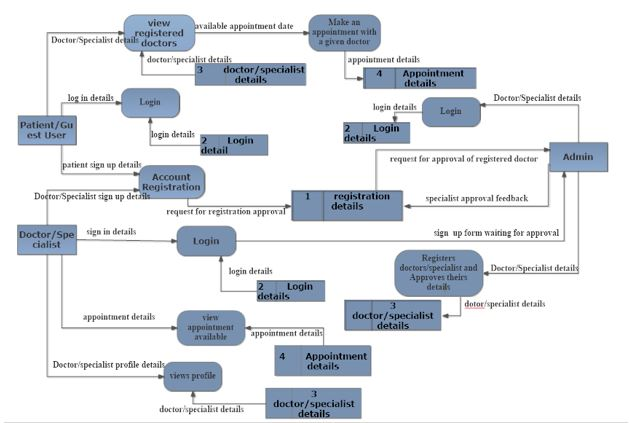
\includegraphics[scale=1.2]{dfd}
\end{center}

\paragraph{•}Chapter 5

\section{System implementation and testing}

\subsection{Introduction} 
\paragraph{•}This chapter best describes the various modules involved in the development and functionality of the system. This Chapter shows screen shots of the system interfaces and also explain the programming environment, data manipulation, form input design and the scripting which was used during the implementation stage of Web Application system.

\subsection{Implementation tools} 
\paragraph{•}The relations between the entities were created using a script that runs on a database that was created using MySQL workbench for MySQL and primary keys uniquely identifying all the entities and checks duplication while foreign keys link tables and enhance referential integrity. Data manipulation that is inserting, deleting, retrieving and ordering for outputs for any search was done at this level.
\paragraph{•}The system was designed in windows to ensure easy adaptation and maintainability. On the server side, MySQL and PHP scripting languages were used to manage the database structure because of its fast processing with the fact that the database is accessed over internet.
\paragraph{•}Expansion of the internet came after the introduction of globally unique identifier to digital information (URL), the development of HTML and the compilation of HTTP and forming World Wide Web in early 1990s. This means that since it is possible to access the information on the network, the HTML was used to design the app pages.
\paragraph{•}SQL was used in the data manipulation i.e. inserting, deleting, retrieving and ordering of outputs for any search. 
JavaScript was used to organize client side functionalities and its functionality.

\subsubsection{Interface} 
\paragraph{•}The interfaces were designed using Hyper Text Mark-up Language 5 (HTML5). This makes up the overall graphical user interface in which JavaScript was embedded to give client side effect with all its functionality and to trigger the right PHP scripts on the server with the appropriate SQL queries that fetch data from MySQL database

\subsubsection{Form Inputs} 
\paragraph{•}MySQL and PHP were used to enter data, change data and HTML5 along with CSS and JavaScript to view data. Forms offer the most convenient layout for entering, changing and viewing data. The following are the forms that were created; signup form and login form.

\subsection{Results or system functionalities}
\paragraph{•}The following screenshots are to explain the different user interfaces available in the proposed system which include the user login, appointment module,home page.


\subsubsection{Patients / Users Home Page} 
\paragraph{•}Displays a welcome message created by the administrator. Links to view article details are shown. Login is shown on the top menu if user has not logged in.

\begin{center}
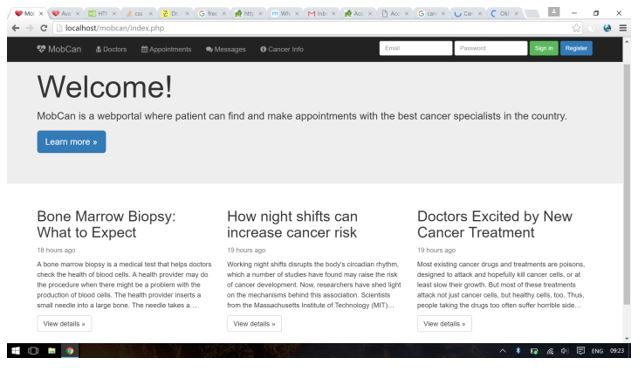
\includegraphics[scale=1.2]{home}
\end{center}


\subsubsection{login}
User must be logged in to complete the appointment booking

\begin{center}
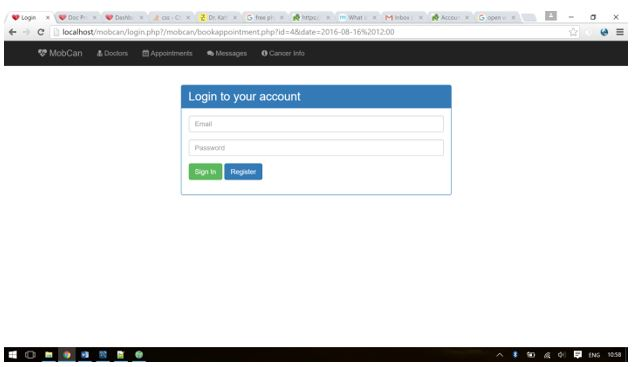
\includegraphics[scale=1.2]{login}
\end{center}

\subsubsection{Appointment page}


\begin{center}
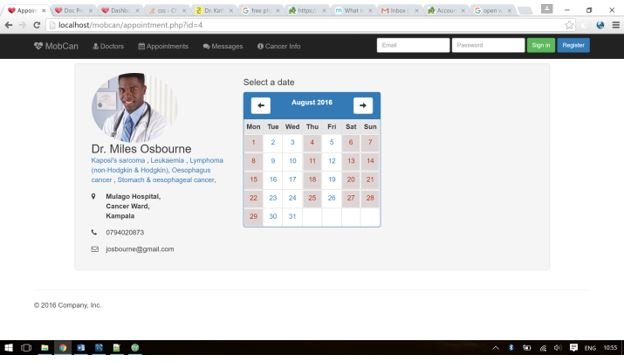
\includegraphics[scale=1.2]{appointment}
\end{center}


\begin{thebibliography}{9}

\bibitem{Timmreck} Prof. Timmreck. \textit{Demographic and Clinical Profile of Cancer Patients },Internet:https://awlworld.com/demographic-and-clinical-profile-of-cancer-patients-and-their-psychosocial-needs, August 26, 2017[April 18, 2018].


\bibitem{Carr} 
Carr-Schmid A, Pfund C, Craig EA, Kinzy TG. \textit{SGD},Internet:https://www.yeastgenome.org/reference/S000069709, August 26, 2013[April 18, 2018].

\bibitem{Hewitt}J Pers Soc Psychol. \textit{NCBI},Internet:https://www.ncbi.nlm.nih.gov/pubmed/12793591, June 6, 2003[April 18, 2018].



\end{thebibliography}







\paragraph{•}APPENDIX
\paragraph{•} i. Projected Cost For Development

\begin{center}
\begin{tabular}{|l|l|l|c|}
\hline NUMBER  & ACTIVITY & COST(Shs) \\\hline

1 & Gathering information & 150,000 \\\hline
2 & Design a framework & 100,000\\\hline
3 &Implementation & 200,000 \\\hline
4 & Stationary & 50,000\\\hline
5 & Transport & 120,000\\\hline
6 & Miscellaneous & 200,000\\\hline
  & TOTAL & 820,000\\\hline
\end{tabular}
\end{center}

\paragraph{•} ii.QUESTIONNAIRES
\paragraph{•}1. How long have you noticed the bone pain?
\paragraph{•}Why: to establish if acute or chronic.


\paragraph{•}2. Is the bone pain localized or generalized?

\paragraph{•}3. If localised, where is the bone pain?

\paragraph{•}4. Is there a history of trauma or injury?
\paragraph{•}Why: may suggest fracture. If the injury was minimal may suggest osteoporosis or pathological fracture due to bone tumour or bone metastases.

\paragraph{•}5. Is the bone pain present day at night?
\paragraph{•}Why: may suggest more serious cause such as bone tumour, bone metastases, leukaemia, Paget's.


\paragraph{•}Fever
\paragraph{•}Why: may suggest osteomyelitis, infective discitis.


\paragraph{•}7. Is there a limitation of motion of the joints?
\paragraph{•}Why: may indicate Osteoarthritis, Rheumatoid arthritis or ankylosing spondylitis, bone tumours, osteomyelitis or fracture.

\paragraph{•}8. Symptoms of bone metastases?
\paragraph{•}Why: e.g. malaise, fever, weight loss, pathological fractures.

\paragraph{•}9. Symptoms of multiple myeloma?
\paragraph{•}Why: e.g. bone pain, usually back ache, symptoms of anaemia, recurrent infections, and symptoms of renal failure.


\paragraph{•}10. Symptoms of Paget's disease?
\paragraph{•}Why: e.g. deformed bone, warm skin over affected area, enlargement of skull, persistent headaches.




\end{document}
